% ================================================================
% CHAPTER 3.1: Domänenanalyse: Literaturrecherche
% ================================================================
\section{Literaturrecherche}
\subsection{Grundlegende Geburtsanzeichen}

Zahlreiche Anzeichen liefern Hinweise auf eine bevorstehende Geburt eine Kalbes. Diese Anzeichen umfassen sowohl bestimmte Positionen und Bewegungsabläufe der Kuh als auch klarer oder blutiger Scheidenausfluss \citep[S. 1]{Lange2017}.

Verdächtige Bewegungsabläufe als Anzeichen für eine bevorstehende Entbindung sind wiederkehrende Schwanzhebung, häufiges Trippeln oder die Drehung des Kopfes zum Bauch hin \citep[S. 1]{Lange2017}. Auch wiederholtes Aufstehen und Abliegen sind Geburtsanzeichen \citep[S. 4]{Saint-Dizier2015}. Das seitliche Liegen mit Abdominalkontraktion stellt eine verdächtige Position dar \citep[S. 1]{Lange2017}. 

Weitere Geburtsanzeichen können eingefallene Beckenbänder, ein \gls{Oedem}\footnote{\label{glossar-oedem}siehe Glossar} am Euter, glänzende Zitzen oder tropfende Milch sein. Auch eine rote Färbung der  äusseren Geschlechtsorgane mit zäher Schleimspur liefert Hinweise auf eine Entbindung \citep[S. 6]{Traulsen2013}. Zudem weisen \gls{Hyperplasie}\footref{glossar-oedem} des Euters, Schamlippenödem und \gls{Sekret}\footref{glossar-oedem} von Schleim auf eine bevorstehende Geburt hin \citep[S. 2]{Streyl2011}.

\begin{figure}[H]
	\center
	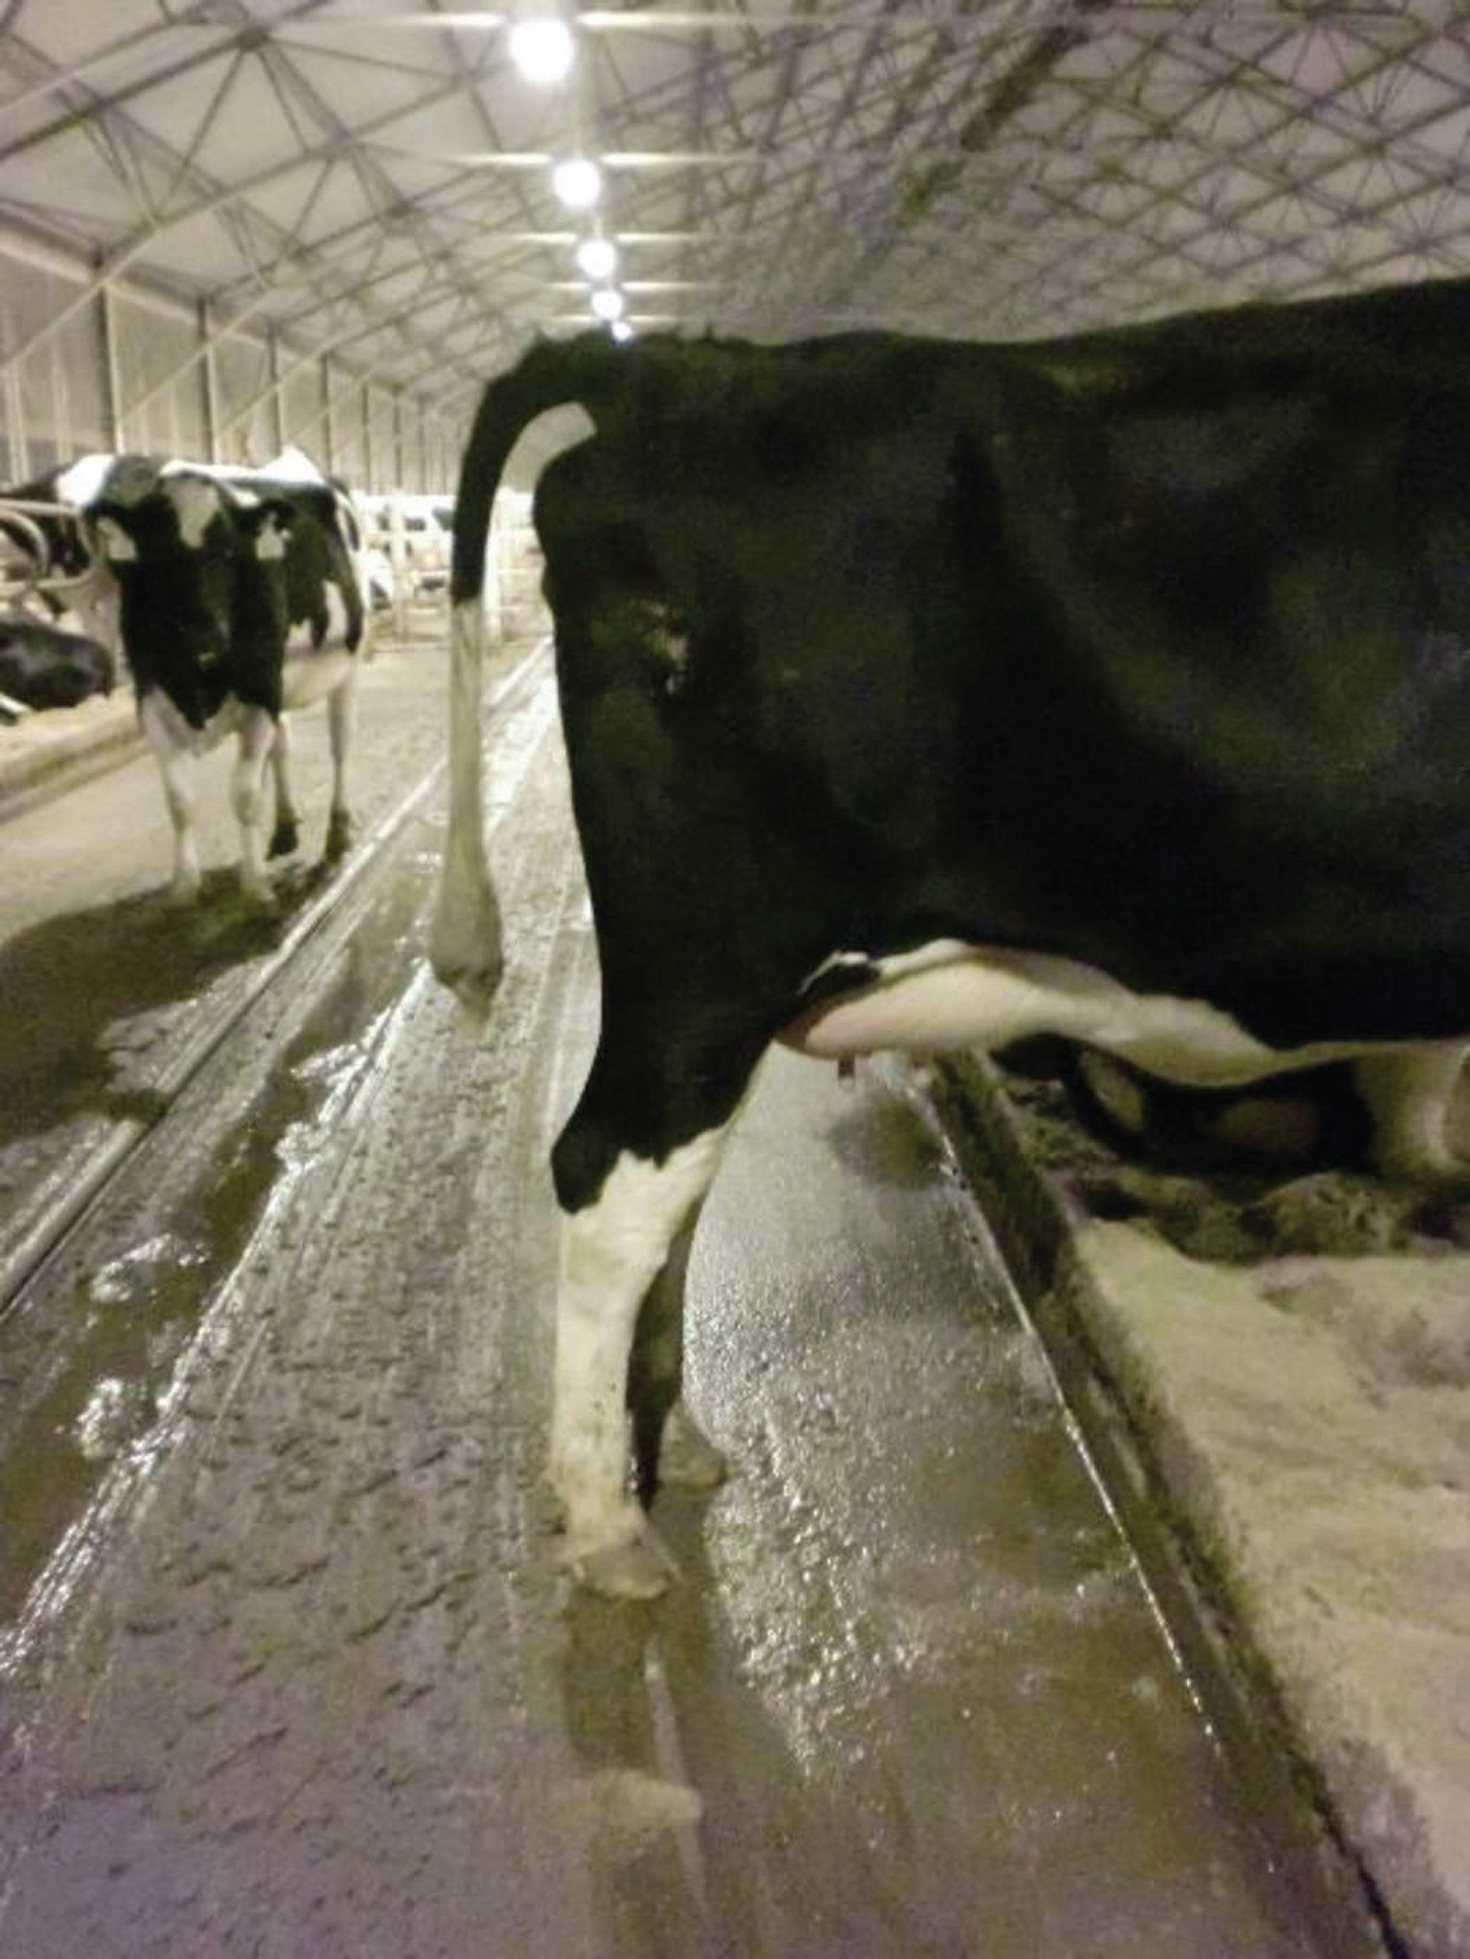
\includegraphics[scale=.45]{Grafiken/schwanzhebung.jpg}
	\caption{Schwanzhebung}
	\label{fig: Schwanzhebung}
\end{figure}

Schwanzhebung wie in Abbildung  \ref{fig: Schwanzhebung} von Lange et al. tritt vermehrt in den letzten $24$ Stunden vor dem Kalben auf \cite[S. 1 f.]{Lange2017}.
\subsection{Zeitliche und prädiktive Hinweise zu den Geburtsanzeichen}
Es ist zu beachten, dass einige Hinweise in erster Linie auf eine Entbindung innerhalb der nächsten vier Tage hinweisen (nachfolgend Vorkalbeperiode genannt), während andere Anzeichen auf eine Geburt innerhalb der nächsten $24$ Stunden hinweisen. Ruhelosigkeit, wiederkehrende Schwanzhebung und die Drehung des Kopfes zum Bauch hin treten häufig $12$ bis $6$ Stunden vor der Geburt auf. Scheidenausfluss weist darauf hin, dass innerhalb der nächsten $6$ Stunden die Geburt eintritt. \citep[S. 1]{Lange2017}

Bereits durchgeführte Experimente von \citep[S. 1]{Lange2017} anhand von stündlicher Beobachtung konnten das Kalben nicht präzise vorhersagen. Demgegenüber konnte das Kalben für die nächsten $12$ Stunden jedoch mit hoher Wahrscheinlichkeit ausgeschlossen werden ($88.5$ bis $97.1$ Prozent). Mit der Information, dass eine Kuh in den nächsten $12$ Stunden nicht kalben wird, können Zeit und Ressourcen bei der Überwachung optimiert werden. Daher sind auch Merkmale zu definieren, welche darauf hinweisen, dass \textit{keine} Geburt stattfindet.

Die wichtigsten Parameter zur Prognose des Kalbens innerhalb der nächsten $12$ Stunden sind Beckenbänder, Zitzenfüllung, \gls{Aufeutern}\footnote{\label{glossar-aufeutern}siehe Glossar} und Scheiden- und Euterödeme. Diese Parameter erlauben eine genaue Vorhersage des Ausbleiben des Kalbens \citep[S. 4]{Streyl2011}.



\begin{figure}[H]
	\center
	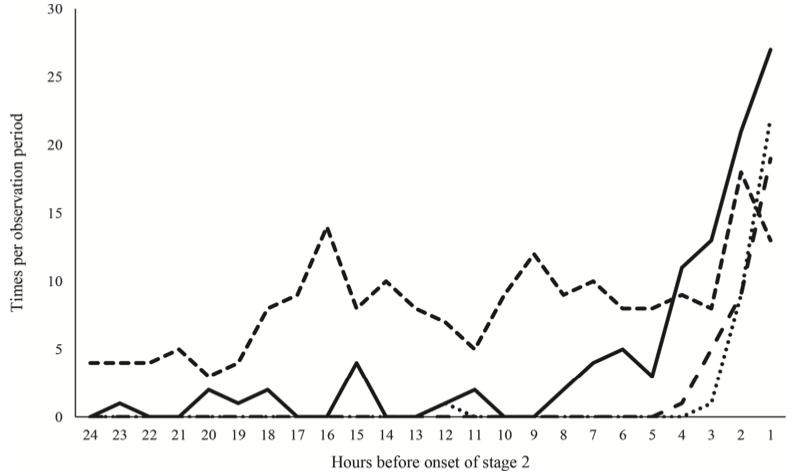
\includegraphics[scale=.45]{Grafiken/observationTimes.png}
	\caption{Häufigkeit von Geburtsanzeichen während den letzten $24$ Stunden vor Geburtsstadium zwei \citep[S.5]{Lange2017}.}
	\label{fig: Häufigkeit von Geburtsanzeichen }
\end{figure}

Die Abbildung \ref{fig: Häufigkeit von Geburtsanzeichen } von Lange et al. zeigt Schwanzhebung als durchgezogene Linie, klarer Scheidenausfluss als kurze gestrichelte Linie,  blutiger Scheidenausfluss als lange gestrichelte Linie und seitliches Liegen mit Abdominalkontraktion als gepunktete Linie
\subsection{Weiterführende Geburtsanzeichen}
Die Geburt eines Kalbs wird durch die \gls{Hypothalamus}\footref{glossar-aufeutern}-\gls{Hypophyse}\footref{glossar-aufeutern}-Nebennieren-rinden-Achse des \gls{Foetus}\footref{glossar-aufeutern} gesteuert. $72$ Stunden vor der Geburt des Kalbs können diverse hormonelle Veränderungen beobachtet werden. Beispielsweise nimmt die \gls{Fetal}\footref{glossar-aufeutern} Produktion von \gls{Kortisol}\footref{glossar-aufeutern} ungefähr $10$ Tage vor der Geburt stark zu, was wiederum das \gls{Progesteron}\footref{glossar-aufeutern}-\gls{Oestradiol}\footref{glossar-aufeutern}-Verhältnis im mütterlichen Blut beeinflusst. Auch Informationen zur Veränderung der Temperatur der äusseren Geschlechtsorgane und zum Wiederkauverhalten können für sensorbasierte Systeme einen deutlichen Mehrwert in Bezug auf die prädiktive Analyse schaffen. Ausserdem versuchen Kühe am Tag der Geburt vermehrt, sich von der Herde zu isolieren \citep[S.1-4]{Saint-Dizier2015}. 
Da die vorliegende Arbeit aber auf die Analyse von Bildern fokussiert, werden diese sozialen Merkmale in der nachfolgenden Arbeit nicht mehr thematisiert. 
\subsection{Ablauf einer normalen Geburt}
Normalerweise befinden sich Kälber in der Vorderendlage. Das heisst, dass zuerst die Vorderbeine und der Kopf durch die Scham gepresst werden \citep{Muller2020}. Eine mögliche Fehlhaltung\footnote{Der zitierte Bericht \glqq Geburtsüberwachung und Geburtshilfe beim Rind\grqq{} veranschaulicht die Fehlhaltungen und mögliche Eingriffe durch Landwirte und Tierärzte.} ist die Hinterendlage. In diesem Fall wird das Kalb mit den Hinterbeinen voran abgekalbert. Weiter stellen Kopfseitenhaltung, Rückenquerlage und gebeugte Gliedmassen ein Risiko für die Geburt dar. Bei der Rückenquerlage ist in der Regel ein Kaiserschnitt notwendig. Die übrigen Fehlhaltungen sind oftmals durch den Landwirten korrigierbar \citep[S. 17, 24-26]{Traulsen2013}.

\begin{figure}[H]
	\center
	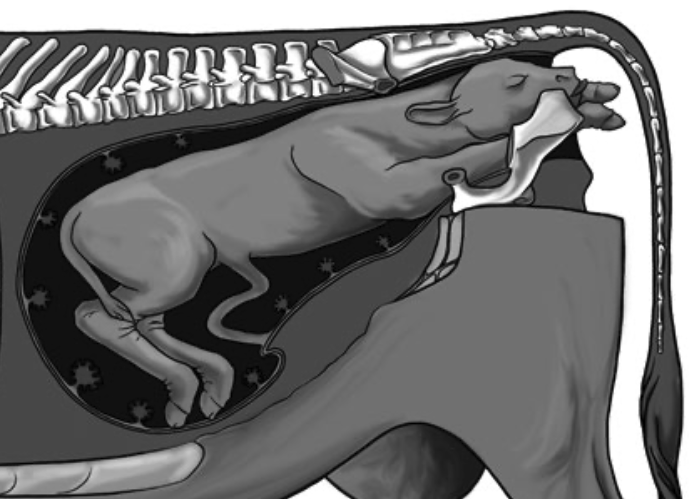
\includegraphics[scale=.45]{Grafiken/vorderendlage.png}
	\caption{Veranschaulichung zur Vorderendlage eines Kalbes \citep[S. 17]{Traulsen2013}.}
	\label{fig: Schwanzhebung}
\end{figure}

Eine Geburt kann in fünf Phasen eingeteilt werden: Vorbereitungsphase, Öffnungsphase, Aufweitungsphase, Austreibungsphase und Nachgeburtsphase \citep[S. 6-8 ]{Traulsen2013}.

In der Vorbereitungsphase stellt sich die Kuh auf die bevorstehende Geburt ein. Deshalb treten die obengenannten Geburtsanzeichen auf. Zwei wichtige Merkmale sind eingefallene Beckenbänder oder rote Färbung der äusseren Geschlechtsorgane \citep[S. 6 ]{Traulsen2013}.  

Die Öffnungsphase erstreckt sich über $6$ bis $16$ Stunden. Der innere Muttermund öffnet sich und die Fruchtblasen treten in den Gebärmutterhals ein, damit dieser gedehnt wird. Es treten erste, leichte Wehen auf und die Kuh kann unruhig sein \citep[S. 7 ]{Traulsen2013}.  

\begin{figure}[H]
	\center
	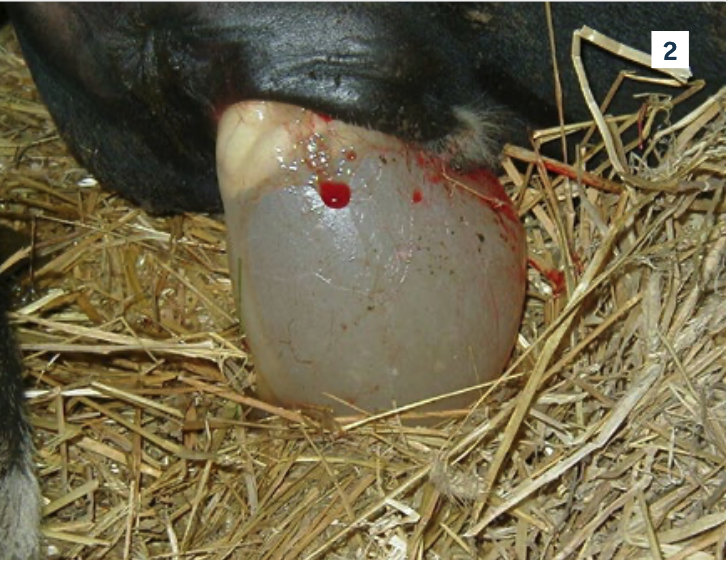
\includegraphics[scale=.45]{Grafiken/oeffnungsphase.png}
	\caption{Wasser- und Schleimblase}
	\label{fig: Öffnungsphase}
\end{figure}

In Abbildung \ref{fig: Öffnungsphase} weiten die Fruchtblasen (Wasser- und Schleimblase) bei der Öffnungsphase den Geburtsweg \citep[S. 7 ]{Traulsen2013}. 

Die Zeit vom Blasensprung bis zum Durchtreten des Kopfes wird als Aufweitungsphase bezeichnet und dauert $1$ bis $6$ Stunden \citep[S. 7 ]{Traulsen2013}. 
\begin{figure}[H]
	\center
	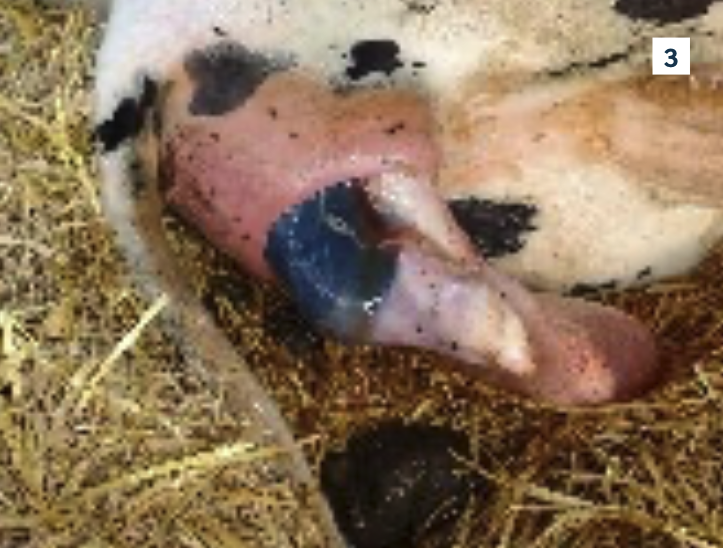
\includegraphics[scale=.45]{Grafiken/aufweitungsphase.png}
	\caption{ Aufweitungsphase }
	\label{fig: Aufweitungsphase}
\end{figure} 

Die Aufweitungsphase ist in Abbildung \ref{fig: Aufweitungsphase} sichtbar und dauert bei Kühen im Normalfall $1$ bis $3$ Stunden. Bei Färsen kann dies bis zu $3$ Stunden länger dauern. \citep[S. 7 ]{Traulsen2013}

Im Rahmen der Austreibungsphase sollte das Kalb in nur $5$ bis $15$ Minuten nach dem Durchtritt des Kopfes durch die Scham geboren sein \citep[S. 8 ]{Traulsen2013}.  


\begin{figure}[H]
	\center
	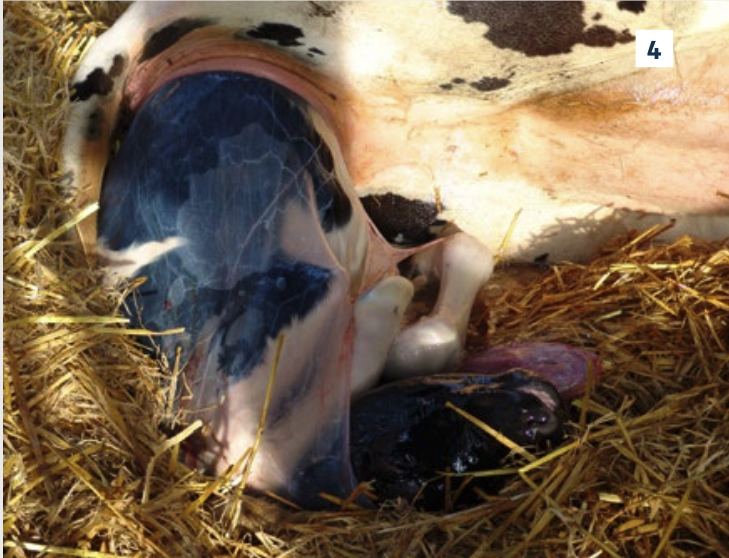
\includegraphics[scale=.45]{Grafiken/austreibungsphase.png}
	\caption{Austreibungsphase}
	\label{fig: Austreibungsphase}
\end{figure}

 In der Austreibungsphase (Abbildung \ref{fig: Austreibungsphase}) wird das Kalb zur Welt gebracht \citep[S. 8 ]{Traulsen2013}

Die Nachgeburtsphase dauert $6$ bis $12$ Stunden und dabei verliert die Kuh das restliche Fruchtwasser und die Nachgeburt \citep[S. 8 ]{Traulsen2013}.  
